\documentclass[a4paper,11pt]{article}
\usepackage{xcolor}
\usepackage{tikz}
\usetikzlibrary{shapes.arrows,arrows.meta}
\begin{document}
\begin{figure}[h!]
    \scalebox{0.08}{
    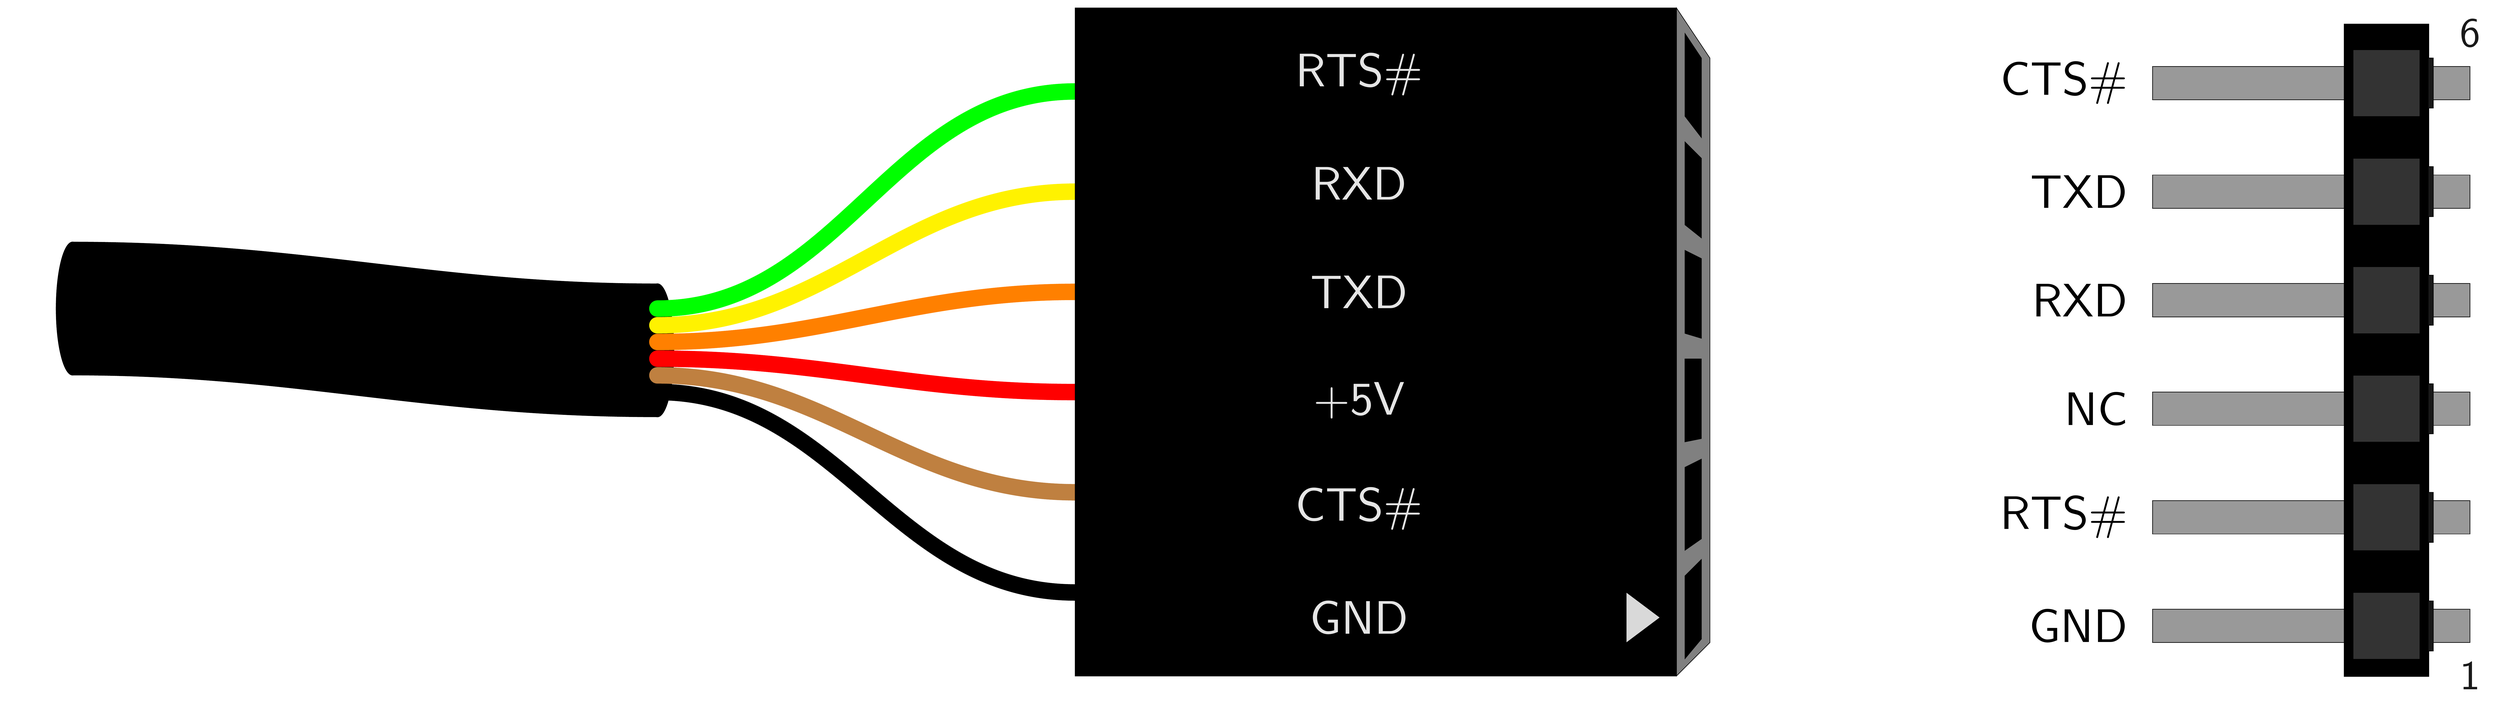
\begin{tikzpicture}[font=\sffamily]
 	\foreach \p [count=\q from 0] in {{GND},{RTS\char"0023},{NC},{RXD},{TXD},{CTS\char"0023}}{
  		\draw[line width=1, fill=gray!80] (4.5, 0+\q*6.5) rectangle ++(19,2) {};
		\draw (-1, 1+\q*6.5) node[scale=8,text width=1cm,align=right]{\p};   		
   	}   	
   	\draw[line width=1mm, fill=black] (16, -2) rectangle ++(5,39) {};
  	\foreach \i in {0,...,5} {
  	   	\draw[line width=1, fill=black!80] (16.5,-1+\i*6.5) rectangle ++(4,4) {};
 	   	\draw[line width=1, fill=black!90] (21,-0.5+\i*6.5) rectangle ++(0.3,3);
  	}
	\draw (23.5,36.5) node[scale=7,black!90]{6};
	\draw (23.5,-2) node[scale=7,black!90]{1};
	
	\draw[line width=1,fill=black](-60,-2) rectangle ++(36,40){};
	\draw[line width=1,fill=gray](-24,-2) -- ++(2,2) -- ++(0,35) -- ++(-2,3) -- cycle;
	
	\draw[fill=black] (-85,17.5) ellipse (1cm and 4cm);
	\draw[fill=black] (-120,20) ellipse (1cm and 4cm);
	\draw[line width=8cm] (-85,17.5) to [out=180,in=0] (-120,20);
	%\draw (-121,12) node[scale=10] (arrow) {$\leftarrow$};
	%\node[scale=10, below of=arrow, node distance=1em] {USB};
	
 	\foreach \p/\c [count=\q from 0] in {{RTS\char"0023}/{green},{RXD}/{yellow},{TXD}/{orange},{+5V}/{red},{CTS\char"0023}/{brown},{GND}/{black}} {
  		\draw[fill=black](-23.5,-1+6.5*\q) -- (-23.5,4+6.5*\q) -- (-22.5,5+6*\q) -- (-22.5,0.2+6*\q);
		\draw (-43, 34-\q*6.5) node[scale=8,text width=1cm,align=center,text=gray!20]{\p};   	
		\draw[line width=28,line cap=round,color=\c] (-60,33-\q*6) to [out=180,in=0] (-85,20-\q);	
   	}   	
	\draw[fill=gray!30] (-27,0) -- ++(0,3) -- ++(2,-1.5) -- cycle;
	\draw[line width=1,fill=black](-60,-2) rectangle ++(2,40){};
	
    \end{tikzpicture}
    }
    \caption{TTL Pin Header}
    \label{fig:ttlpins}
\end{figure}
\end{document} 



